% !TEX TS-program = xelatex
% !TEX encoding = UTF-8 Unicode
% !Mode:: "TeX:UTF-8"

\documentclass{../../styles/resume}
\usepackage{../../styles/zh_CN-Adobefonts_external} % Simplified Chinese Support using external fonts (./fonts/zh_CN-Adobe/)
%\usepackage{../../styles/zh_CN-Adobefonts_internal} % Simplified Chinese Support using system fonts
\usepackage{../../styles/linespacing_fix} % disable extra space before next section
\usepackage{indentfirst}
\usepackage{cite}


\begin{document}

\pagenumbering{gobble} % suppress displaying page number

\begin{center}
  \begin{minipage}{\textwidth}
    \centering
    \name{Who Am I}
    \vspace{0.1em}
    \basicInfo{
      \email{w*********@gmail.com} \textperiodcentered\ 
      \phone{(+86) 178-****-****}
    }
    \basicInfo{
      {男 | 山西省晋城市 | 中共预备党员}
    }
  \end{minipage}
\end{center}


\begin{tikzpicture}[remember picture, overlay]
  \node[anchor=north east, inner sep=0pt] at ([xshift=-1.5cm, yshift=-1.5cm]current page.north east) {
    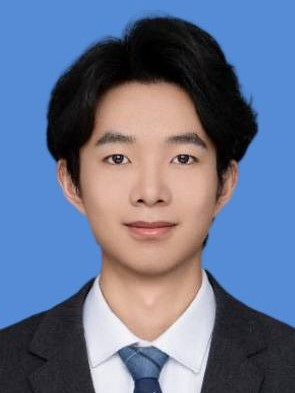
\includegraphics[width=1in]{../../assets/images/一寸.jpg}
  };
\end{tikzpicture}

\section{\faGraduationCap\ 教育背景}
\begin{itemize}
  \item \textit{武汉大学计算机学院软件工程}\ 22级本科在读
  \item \textit{GPA:} 3.852/4.0 \quad\quad \textit{排名:} 26/235 (11.02\%)
    \item\textit{主修课程: }\ 数据结构(93),离散数学(95),⾼级语⾔程序设计(95),系统级程序设计(94),系统级程序设计(93),高等数学(97),概率论与数理统计(95)
\end{itemize}
% 系统级程序设计(95),概率论与数理统计(95),

\section{\faUsers\ 项目经历}
\datedsubsection{\textbf{训练基于文本相似度计算的软件故障定位模型}}{2024年4月}
\role{软件测试与故障定位}{Python, NLP, IR}
\begin{onehalfspacing}
利用软件变更(即代码提交记录)来定位缺陷
\begin{itemize}
  \item 软件变更记录了代码的修改历史,包括变更的意图、修改的代码片段以及变更的上下文信息
  \item 代码块变更的粒度比文件更细,调试时可以显著减少需要检查的代码量
  \item 构建基于自然语言和代码实体的两个语料库,并使用VSM对变更历史进行索引和排名
\end{itemize}
\end{onehalfspacing}
% 职业技能匹配系统项
\datedsubsection{\textbf{职业技能匹配系统}}{2024年10月}
\role{湖北省大学生创新创业项目}{vue+Springboot, Python, NLP}
\begin{onehalfspacing}%下面一行总述
对职位描述和求职者信息进行语义分析和匹配,以实现精准的职位推荐
\begin{itemize}%这里都是分点
\item 分析用户上传的简历并提取关键信息
\item 提取多平台招聘信息并依据职位要求进行文本多分类
\item CNN模型与ERNIE语义网络的简历职位匹配算法
\end{itemize}
\end{onehalfspacing}



\datedsubsection{\textbf{大语言模型相关方向科研实习}}{2025年2月}
\role{科研实习, 文献调研与技术分析}{Python, Literature Review}
\begin{onehalfspacing}
阅读学习文献,围绕LLM-Agent 架构与 LLM 评估方法展开探索
\begin{itemize}
  \item 基于开源框架搭建了基础的 Agent 系统,实现简单的任务调度与反馈机制
  \item 对比不同模型在特定任务上的表现,初步掌握了一套科学的大语言模型评估方法
\end{itemize}
\end{onehalfspacing}


\section{\faHeartO\ 曾获荣誉}
\datedline{\textit{2023年全国大学生数学竞赛 湖北省一等奖}}{2023年12月}
\datedline{\textit{2025年第十六届蓝桥杯大赛C/C++程序设计 湖北省二等奖}}{2025年04月}
\datedline{\textit{2024-2025学年国家励志奖学金}}{2024年10月}
\datedline{\textit{2024-2025学年武汉大学优秀学生乙等奖学金}}{2024年10月}
\datedline{\textit{2024-2025学年武汉大学三好学生}}{2024年10月}


\section{\faInfo\ 个人情况总结}
\begin{itemize}
  \item \textit{英语能力:} 英语六级547分,具备不错的听说读写能力,熟练阅读英文学术文献
  \item \textit{编程技能:} 熟练掌握Python、Java、C/C++,熟悉numpy、torch等用法
  \item \textit{技术领域:} 自然语言处理、深度学习、前后端开发、图像处理、语义分析
  \item \textit{身心健康:} 热爱长跑和魔方运动,数次参加马拉松比赛以及武汉市内魔方比赛
  \item \textit{综合素质:} 具备扎实的数学基础、严谨的科研素养、团队协作与创新能力
\end{itemize}


\end{document}
